%============================================================
\section{Nombre: Embestida aerea.}\label{hab.EmbesAer}
\subsection{Descripción}
El enemigo usara este ataque cuando este lejos del jugador. El enemigo arremeterá a gran velocidad contra el jugador siguiendo una trayectoria de diagonal descendente.
\subsection{Portador}
Itzpápalotl (ver apartado \ref{per:itzpapalotl}).
\subsection{Esquema}
			Ver figura \ref{fig:embestidaA}.
			\begin{figure}
				\centering
				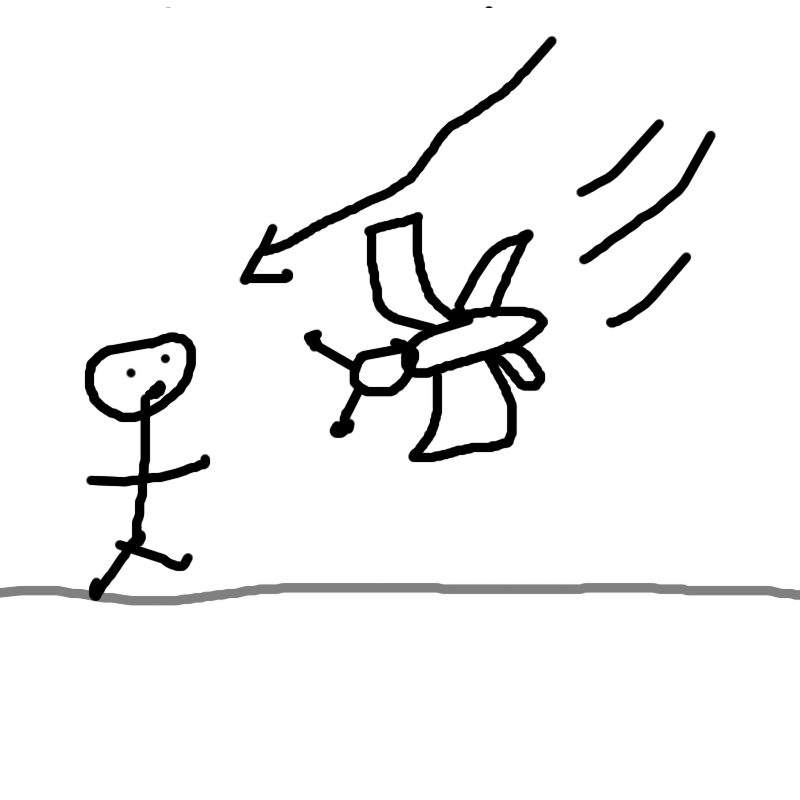
\includegraphics[height=0.2 \textheight]{Imagenes/embestidaA}
				\caption{Embestida aerea.}
				\label{fig:embestidaA}
			\end{figure}